\chapter{Migration Jira/Java Correction WorkBench}\label{chapitre:migration}

\section{Qu'est-ce que Jira et Java Correction WorkBench (JCWB)}
Jira\index{Jira} est un logiciel de tra\c{c}abilit\'{e} des probl\`{e}mes d\'{e}veloppé par Atlassian dont l'usage est gratuit pour les organisations \`{a} but non lucratif, de charit\'{e} ou les projets open-source. SAP désire migrer de système de traçabilité pour utiliser maintenant Java Correction WorkBench\index{Java Correction WorkBench} (JCWB ou CWB).\\

JCWB est un logiciel interne à SAP dont l'utilisation à été imposée par la hiérarchie, son domaine d'utilisation est la gestion des corrections. Historiquement, SAP utilise Jira pour gérer le projet, les problèmes (defects) et les corrections.\\
La stratégie de gestion des bugs changeant, SAP a pris la décision d'utiliser un seul et même outil de gestion des problèmes en interne comme en externe (à l'usage des clients) : BCP. Cet outil permet de renseigner un problème, quel qu'il soit, et s'il s'avère que ce problème est un bug logiciel il est transféré vers JCWB, qui suivra ce bug toute la durée de la correction.

%ASTEC est un logiciel interne à SAP dont la première version est sortie en 2007. ASTEC



\section{Pr\'{e}sentation du contexte}


\`{A} SAP, tous les codes des différents projets sont hébergés sur le gestionnaire de version Perforce\index{Perforce} (SCM : Source Code Management)
et ceux-ci sont compilés plusieurs fois par jour grâce à Jenkins\index{Jenkins} (CIS : Continuous Integration Software).\\
Chaque projet est constitué de deux choses distinctes, d'une part, son code source et, d'autre part, les tests joués pour garantir\footnote{La valeur de la garantie dépend directement du test coverage} le bon fonctionnement du produit. Lorsqu'il y a un problème sur la build, que ce soit une erreur de compilation ou un test qui échoue, le statut de la build change pour être représentatif du problème. Dès lors que quelqu'un s'en aperçoit, il inscrit un defect\index{Defect} dans Jira\footnote{L'utilité de Jira est bien plus large que la simple déclaration d'un test échoué, il sert à décrire n'importe quel problème quelle que soit la version, la branche ou le produit} ou dans JCWB, en fonction de la nature du problème\\


\section{Plugin de reporting}
Pour leur permettre d'avoir un rapport visuel sur l'état des builds, ils utilisent le plugin Radiator. Ce plugin permet l'affichage, sur un seul écran divisé, des groupes de jobs\footnote{Typiquement, un job correspond à un projet logiciel}. Un groupe de jobs est représenté par un carré coloré dont la couleur représente l'état des jobs qui le composent, voir la capture d'écran figure \ref{figure:radiatorActual} page \pageref{figure:radiatorActual}.\\
Les statuts pris en compte sont les statuts Jenkins\footnote{Error, Failure, Unstable, Aborted, Not built, Success} ainsi qu'un statut supplémentaire issu du plugin Claim. Ce plugin permet à un développeur de \textquote{claimer} une erreur, c'est-à-dire, ajouter au projet une information supplémentaire : le nom de l'utilisateur qui a \textquote{claimé} et le message que celui-ci a laissé aux autres utilisateurs.




\begin{figure}[!h]
  \centering
      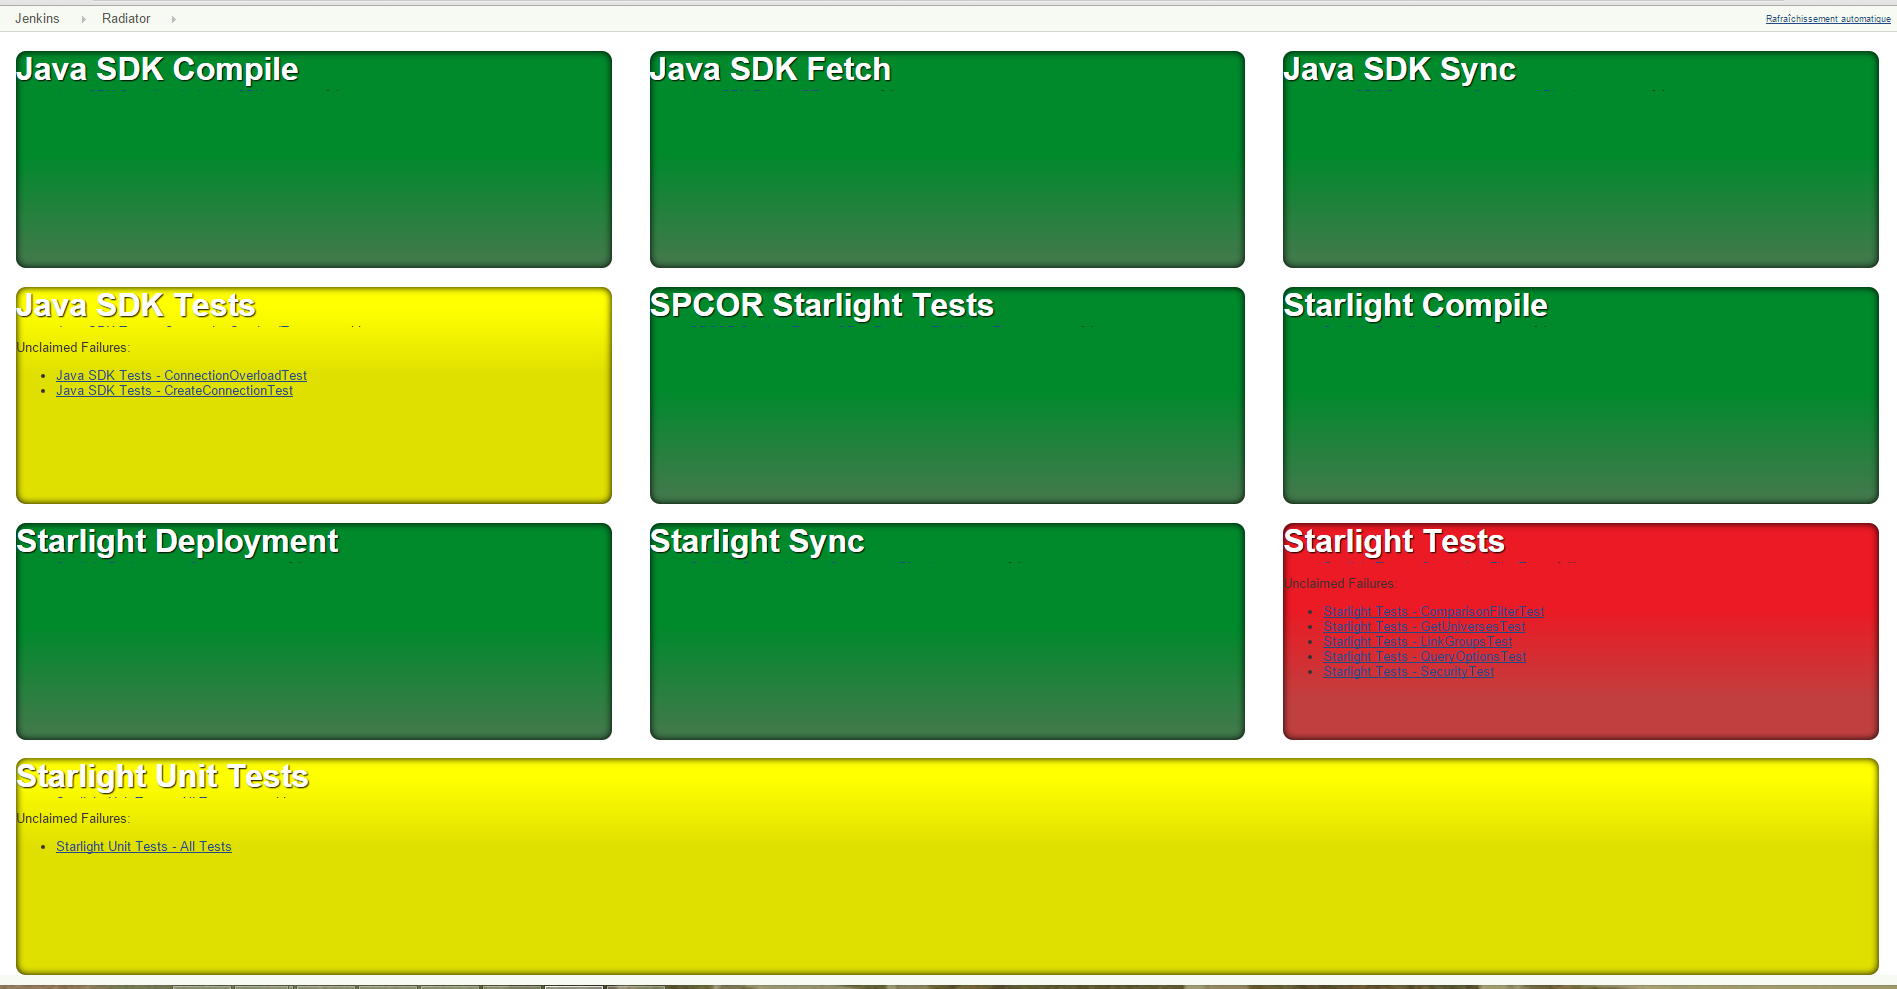
\includegraphics[width=\textwidth]{images/radiatorActual.png}
  \caption{Plugin Radiator utilisé actuellement}
	\label{figure:radiatorActual}
\end{figure}

En résumé Radiator permet de :
\begin{itemize}
	\item rassembler les jobs en un seul groupe de jobs, où chacun des jobs a un statut\footnote{statut propre à Jenkins}
	\item afficher une couleur représentative du statut jugé le plus important
	\item prendre en compte les informations supplémentaires du plugin claim
\end{itemize}
Prennons l'exemple où nous avons deux groupes composés chacun de trois jobs, tous différents. Supposons que, sur les 6 jobs, l'un soit en échec les autres en succès. Nous aurons donc une vue colorée en vert (parce que tous les projets sont en succès) et la deuxième vue colorée en rouge (l'un des jobs ayant échoué) ou bien en orange si l'échec est \textquote{claimé} (échec claim par un développeur).\\
La figure \ref{figure:RadiatorInformationSources} page \pageref{figure:RadiatorInformationSources} illustre bien les sources d'informations du plugin. Il puise ses résultats depuis Jenkins et le plugin claim, les résultats de Jenkins provenant, d'une part, des résultats de tests JUnit, et d'autre part, des compilations, synchronisations vers Perforce, \ldots\\
L'inconvénient de ce procédé est que lorsque qu'un test a échoué, tout le groupe de test passe en rouge. Dans cette situation, il devient impossible de détecter les nouveaux tests qui échouent.




\begin{figure}[!h]
  \centering
      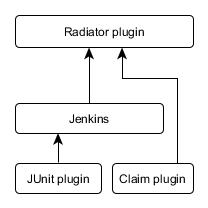
\includegraphics[scale=0.5]{images/RadiatorInformationSources.jpg}
  \caption{Contexte d'utilisation du plugin Radiator utilisé actuellement}
	\label{figure:RadiatorInformationSources}
\end{figure}




La solution simple, mais permettant de contourner le problème et de ne plus polluer l'affichage avec du rouge, consiste à faire passer les jobs en échec avec defect\index{Defect} (ie. reconnus et enregistrés comme échecs dans Jira\index{Jira} ou CWB\index{Java Correction WorkBench}) en vert.\\
De cette manière, puisque seuls les nouveaux échecs apparaissent en rouge, toute régression est visible immédiatement.\\
Cette transformation est mise en \oe{}uvre grâce à une annotation, celle-ci est présentée figure \ref{figure:annotationJava} page \pageref{figure:annotationJava}.\\


\begin{figure}[h]
  \centering
      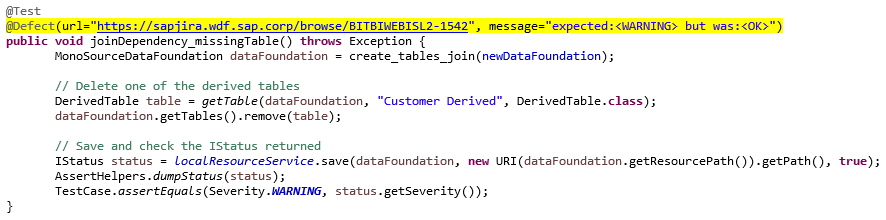
\includegraphics[width=\textwidth]{images/annotationJava.png}
  \caption{Annotation utilisée pour vérifier le statut du defect Jira}
	\label{figure:annotationJava}
\end{figure}

De cette manière le test est relié au defect. \textbf{Et si} :
\begin{enumerate}
	\item le test a échoué mais le statut est \textquote{Active} ou \textquote{Open}
	\item le message d'erreur est de la forme attendue
\end{enumerate}
\textbf{Alors}, le test sera considéré en succès par Jenkins. Ensuite, quand un développeur livrera la correction, le defect passera à \textquote{Validate}, ce qui court-circuitera l'annotation\footnote{même comportement pour le statut \textquote{Closed} ou n'importe quel autre qui n'est pas \textquote{Active} ni \textquote{Open}}. Et en fonction de la validité de la correction, le test redevient vert ou reste rouge.\\
\textbf{De cette manière}, seuls les tests non investigués sont rouges, ce qui permet de réagir beaucoup plus rapidement et réduire le temps d'investigation.\\

Pour résumer, la relation qu'entretien BCP et JCWB est illustrée figure \ref{figure:bugManagementProcess}.

\begin{figure}[h]
  \centering
      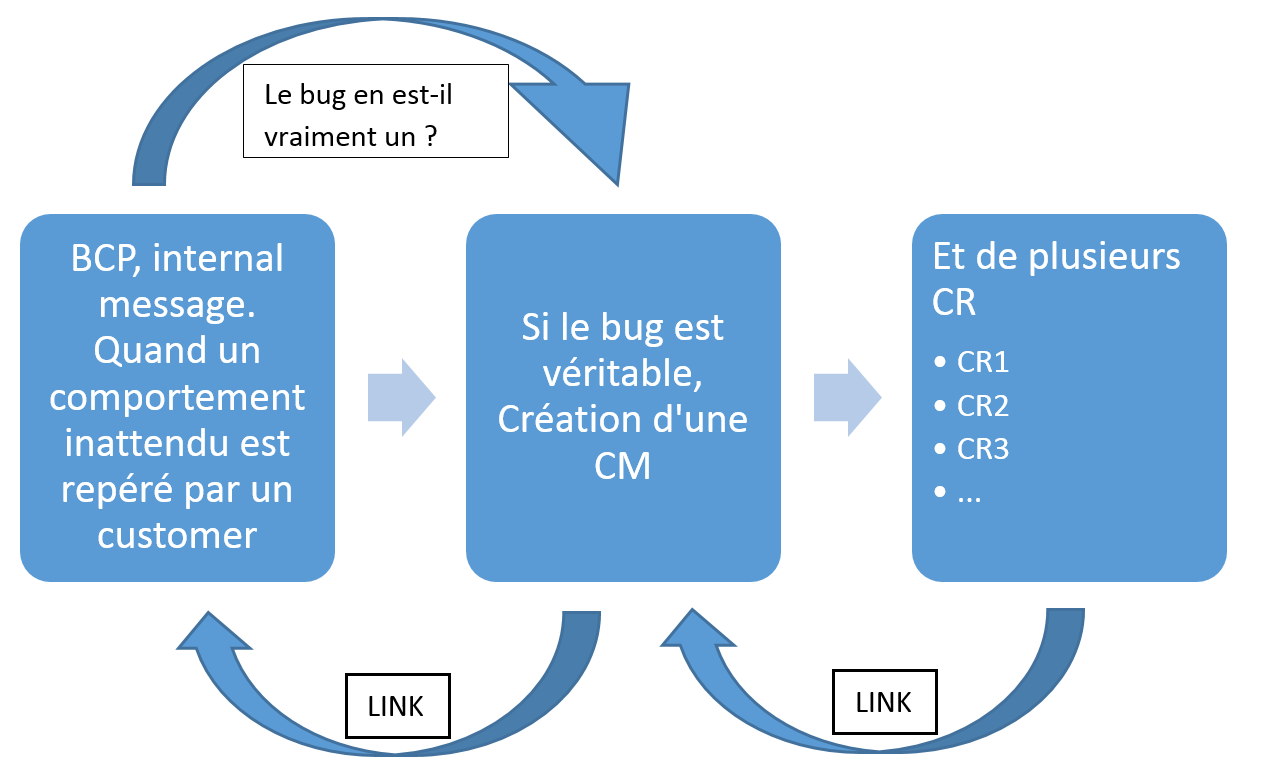
\includegraphics[width=\textwidth]{images/bugManagementProcess.png}
  \caption{Process de gestion de bug utilisé}
	\label{figure:bugManagementProcess}
\end{figure}




\textbf{Probl\'{e}matique}\hfill \\ \indent

Actuellement, seuls les defects rentrés sur Jira sont pris en compte, la mécanique en place ne permet pas de récupérer ces mêmes informations de JCWB\index{Java Correction WorkBench}. \\
Puisque nous ne pouvons pas aller chercher le résultat de JCWB, il faut mettre à jour le process actuel et permettre aux statuts d'être ajustés quelque soit l'origine du defect (Jira ou CWB).\\
La problèmatique supplémentaire relève de l'architecture différente de Jira et de JCWB\footnote{Contient la \textquote{Correction Measure} (CM) et les \textquote{Correction Requests}} (CR), ce qui nous oblige à aller receuillir des informations à deux endroits différents. Le premier objectif étant de récupérer l'identifiant de la \textquote{Correction Request} à laquel le defect est associé et l'identifiant de la \textquote{Correction Measure} à laquelle la CR est associée.\\






\section{Travail effectu\'{e}}


La première partie du travail s'est cantonnée d'abord à des échanges de mails parallèlement à des recherches.\\
La difficulté de cette partie a été de comprendre le problème dans sa globalité. D'abord, je ne connaissais pas le process qui nécessitait cette modification. Dans la partie précédente de mon contrat j'ai pu utiliser Jira\index{Jira} et JCWB\index{Java Correction WorkBench} ainsi que les defects qui y étaient enregistrés, mais c'était tout.
Les différentes choses essentielles à mon projet sont les suivantes :

\begin{itemize}
	\item il existe un web service permettant de récupérer les informations d'une CR : CWB HTTP API
	\begin{itemize}
		\item l'utilisation de ce web service se fait via une authentification normalisée par SAP : PROD-PASS-ACCESS
	\end{itemize}
	\item le fichier à implémenter pour compléter le comportement actuel est JiraIssueWatcher.java	
\end{itemize}




\subsection{Fonctionnement et utilisation de prod-pass-access}
La première chose sur laquelle je me suis penché a été de comprendre le fonctionnement de prod-pass-access, \gls{API} développée par et pour les services de SAP pour sécuriser ses tranferts d'informations.\\
Je suis donc allé sur le portail de l'entreprise pour étudier cette librairie, la première chose que j'ai apprise est que prod-pass-access signifie : \textquote{Production password access} et que son rôle est de lire et écrire des credentials\footnote{Les credentials sont les noms d'utilisateurs ou mots de passe}.\\
Dans les différentes explications que j'ai pu trouver il était indiqué que pour utiliser cette \gls{API} il fallait avoir été, au préalable, enregistré dans un dossier particulier sur un serveur. Je ne comprenais pas grand chose à comment je pouvais utiliser tout ceci, j'ai donc téléchargé l'API en question et ai fait mes expériences en lignes de commande.\\
Je ne connaissais pas cet outil et il me fallait découvrir comment celui-ci fonctionnait car il me permettrait ensuite de communiquer avec le serveur pour pouvoir utiliser l'\gls{API} CWB HTTP API.\\

La documentation de cette API était plutôt claire (figure \ref{figure:prodpassaccessdoc}), et des renseignements ainsi obtenus j'ai pu créer un utilisateur.
\begin{figure}[!h]
  \centering
      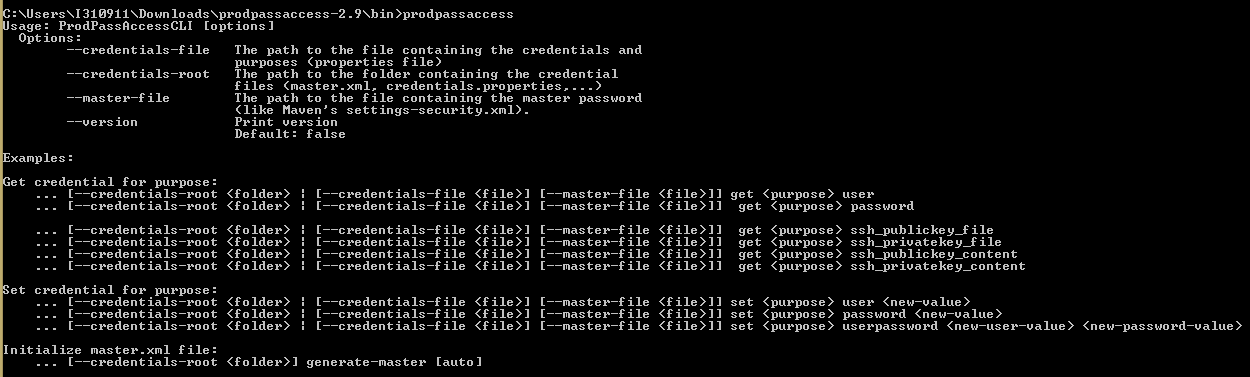
\includegraphics[width=\textwidth]{images/prodpassaccessdoc.png}
  \caption{Documentation fournie par l'API}
	\label{figure:prodpassaccessdoc}
\end{figure}


J'ai suivi les informations me permettant de générer un utilisateur, et au fur et à mesure le fonctionnement de cette API s'est éclairci.\\
Cette API sert à identifier l'utilisateur grâce aux fichiers enregistrés d'une part sur le serveur et d'autre part sur la machine faisant la requête. Les fichiers en local contiennent non seulement le nom d'utilisateur mais aussi le mot de passe en crypté. La clé pouvant décrypter le mot de passe est hébergée sur le serveur et lui seul peut décrypter le mot de passe crypté envoyé par l'utilisateur.

J'ai donc créé mon utilisateur grâce aux commandes suivantes :\\
\begin{lstlisting}
prodpassaccess generate-master 
Prodpassaccess set myPurpose user pierre
Prodpassaccess set MyPurpose password password012
prodpassaccess --credentials-file credentials.properties --master-file master.xml set myPurpose user pierre
\end{lstlisting}

J'ai fait plusieurs tests avant de pouvoir exécuter ces lignes de commandes mais le principe d'utilisation est assez simple.\\
La première ligne va permettre à l'utilisateur de fournir un mot de passe. Après l'exécution, je suis allé voir (comme précisé dans la documentation sur le portail de SAP) dans le dossier prodpassaccess contenu à la racine de mon dossier User, dans celui-ci il y a le fichier master.xml contenant une clé de cryptage.\\
Les deux lignes suivantes permettent de créer un utilisateur et un mot de passe pour un \textquote{purpose} en particulier.\\
La dernière ligne, elle, permet d'enregistrer les informations cryptées dans un fichier \textquote{credentials.properties}..\\
J'avais donc réussi à créer un utilisateur mais je ne savais toujours pas comment l'utiliser dans mon code java. Je me suis donc arrêté là, car je ne pouvais pas tester ce que j'avais réussi à faire.\\







\subsection{Accès au web service}
Maintenant il fallait que je trouve le moyen d'envoyer une requête au \gls{Web service}. Mais avant cela, comme précisé dans la documentation, ce n'était pas une connexion HTTP classique mais SSL nécessitant l'utilisation d'un certificat. Je ne savais pas ce que cela était. J'ai donc discuté avec un collègue ayant déjà utilisé un service similaire et il m'a envoyé un code \gls{Java} qui pourrait m'inspirer. En fouillant dans son code j'ai trouvé une méthode pemettant de passer le contrôle des certificats. Après cela, je pouvais manipuler une connection HTTPS depuis mon code \gls{Java}, mais encore une fois, il ne m'était pas possible de tester le code que j'avais.\\
\`{A} ce moment, je pouvais donc :
\begin{itemize}
	\item utiliser l'API de cryptage des informations : prod-pass-access
	\item me connecter, grâce à une connexion sécurisée, à une url
\end{itemize}
Il me manquait le point essentiel, l'url du web service que je voulais utiliser. Je suis donc aller chercher l'information parmi les membres de mon équipe, ils ne savaient pas non plus, mais m'ont donné le nom de celui qui s'était occupé de développer cette API, un collègue travaillant sur le site de Walldorf, en Allemagne. Je lui ai donc envoyé un mail pour conna\^{i}tre le moyen d'utiliser son API et lui ai demandé sa documentation. Nous avons discuté un peu par mail car celui-ci voulait savoir pourquoi j'en avais besoin et si cela était vraiment nécessaire. Après quelques échanges de mail, celui-ci m'a transmis la documentation relative à l'API dont j'avais besoin.\\
J'ai donc étudié la documentation pour savoir quelle requête je devais envoyer.\\
J'ai trouvé exactement ce qu'il me fallait, il y avait, parmi les différentes méthodes accessibles via le \gls{Web service}, celle qui me retournait le statut de la Correction Request dont l'identifiant est passé en paramètre dans la requête. La requête que je devais envoyé était de la forme :
\begin{lstlisting}
https://css.wdf.sap.corp/sap/bc/bsp/spn/jcwb_api_extern/get_correction_requests?pointer=<id de la correction request>
\end{lstlisting}

J'ai immédiatement essayé cette url que j'ai collé dans la barre d'adresse de mon navigateur avec l'identifiant d'une correction request valide. L'accès à cette url m'affichait uniquement un pop-up me demandant de renseigner un nom d'utilisateur et un mot de passe. J'ai essayé avec mes identifiants personnels que j'utilise tous les jours pour me connecter aux services sécurisés se SAP. La connexion est refusée.\\
C'était donc ici que je devais trouver le moyen d'utiliser les credentials créés grâce à prod-pass-access, et de les intégrer à ma requête HTTPS.\\
J'ai complété mon code \gls{Java} avec l'url du \gls{Web service}. J'ai trouvé dans la documentation de prod-pass-access la marche à suivre pour accéder aux credentials directement depuis mon code \gls{Java}. J'ai donc importé le \gls{JAR} de prod-pass-access dans mon projet.\\
D'autre part, il fallait transmettre les credentials d'une autre façon que par l'url, En étudiant les documentations des requêtes http j'ai trouvé les paramètres qui correspondaient exactement à ce que je cherchais.\\
Le code dont il est question est disponible dans l'annexe \ref{annexe:httpcwbapi} page \pageref{annexe:httpcwbapi}, la solution pour se connecter via HTTPS est implémentée dans la méthode \textquote{sendRequest()} et l'utilisation de l'API ainsi que l'url de l'\gls{API} \textquote{HTTP CWB API} est implémentée dans la méthode \textquote{findStatus()}.

J'ai exécuté mon code contenant tous les éléments pour que cela fonctionne, j'avais tout considéré dans mon code pour me connecter au \gls{Web service} :
\begin{itemize}
	\item j'avais réglé le problème de la connexion sécurisé (protocole SSL)
	\item je pouvais accéder à mes credentials depuis mon code \gls{Java}
	\item j'avais renseigné la bonne url et effectué la bonne requête pour accéder au statut de la Correction Request
	\item j'avais renseigné mes credentials de la manière préconisée par les spécifications du protocole HTTP
\end{itemize}


En réponse, le serveur m'a renvoyé ceci \textquote{{\color{red}ERROR: Bitte übergeben Sie Benutzer und Password}}\\

\subsection{Création du nouvel utilisateur}
\`{A} ce moment je me suis souvenu de la documentation de prod-pass-access, particulièrement d'un élément que je n'avais pas compris quand je l'avais lu pour la première fois. Il s'agissait dans dossier particulier, hébergé sur un serveur à Walldorf. Celui-ci contient tous les credentials des utilisateurs autorisés à utiliser ce service. Je me suis donc repenché sur la création d'un utilisateur et tout se qu'il me restait à faire était de stocker mes informations sur ce serveur en question, et pas en local comme je l'avais fait lors de mes tests.\\
Je suis allé chercher dans la documentation l'adresse de ce fameux dossier pour y enregistrer mes credentials dont l'adresse est 

\begin{lstlisting}
\\production.wdf.sap.corp\info\make\
\end{lstlisting}

Ce dossier contient un grand nombre d'autres dossiers, d'après la documentation, il s'agit de tous les utilisateurs utilisant ce service. J'ai choisi un user générique \textquote{pblack} utilisé par beaucoup d'ingénieurs de chez SAP pour effectuer leurs tests avec ce service. Ce dossier correspond à mon dossier User que j'ai sur ma machine en local. J'ai donc ré-exécuter la commande permettant de stocker les credentials, mais cette fois-ci en précisant le nouvel emplacement.
\begin{lstlisting}
prodpassaccess 
--credentials-file \\production.wdf.sap.corp\info\make\pblack\.prodpassaccess\credentials.properties 
--master-file \\production.wdf.sap.corp\info\make\pblack\.prodpassaccess\master.xml 
set myPurpose pierre 
\end{lstlisting}

Ceci fait, j'ai ré-exécuter mon code \gls{Java} pour me connecter à l'API. La réponse que j'ai reçu était \textquote{Open}, ce qui voulait dire que le statut du defect dont j'avais renseigné l'identifiant dans la requête était toujours en cours de traitement. Mais surtout, cela voulais dire que toute mon implémentation fonctionnait. \\
Je pouvais maintenant revoir mon code, le clarifier et finalement le transmettre pour validation.\\


\section{Conclusion de la mission}
La mission qui m'a été attribué devait compléter le fonctionnement de quelque chose qui existait déjà. Je devais donc, au préalable, étudier le contexte dans le lequel celle-ci s'intégrait. D'autre part, en plus de m'intégrer dans le code déjà existant, je devais intégrer à mon code une API que l'utilisation d'une autre API nécessitait. J'ai appris énormément de choses en Java, même si en terme de lignes de code je n'en ai pas écrit beaucoup, il m'a fallu beaucoup de recherches pour effectuer ce que je voulais, que ce soit au niveau de la sécurité du transfert de données ou des différentes manières de gérer une connexion HTTP en Java. J'ai de plus implémenté une classe abstraite pour la première fois, je n'en avais jamais eu l'utilité et j'ai pu découvrir, par la nécessité, son intérêt et sa puissance. J'ai réussi à obtenir une implémentation fonctionnelle en moins de trois semaines et j'ai été particulièrement ravi d'obtenir ce résultat.



\section{Bilan de cette mission}

J'ai pris beaucoup de plaisir à développer cette solution, bien que ce soit une goutte d'eau parmi l'immensité du Framework de test de Web Intelligence, entrant en jeu dans l'exécution quotidienne des tests.\\
J'ai appris beaucoup de choses en très peu de temps et ai eu le plaisir de travailler avec des inconnus qui étaient mes collègues. Ceux-ci se trouvant en Allemagne, nous avons donc communiqué en anglais, ce petit aspect internationnal de la mission m'a beaucoup plu.\\
Cette mission, bien que très courte, à été très valorisante et enrichissante.\\

Cette mission étant achevée, le fonctionnement du Framework de test s'est maintenant adapté à la migration de logiciel de traçabilité des problèmes.


